\section{Results and Discussion} \label{sec:results}

% @RCK - writing group
% Structure your R&D section to say, for each hypothesis 1. What you're showing. 2. Here's the evidence.
% Combine these figures to support your conclusions.
%
% Think about making two-part figures, one with the time-series, and then a partner panel that has the final dominant comparisons (violin or box plots).
%
% Visually distinguish your figures so that the reader, at a glance, can tell what they're looking at. Consider color-coding the backgrounds, or having distinct plot types for different kinds of conclusions.
%
% If you MUST show a pile of time series, consider combining them into sets of panels. Say one big figure with all your timeseries, but quadrants showing each one as part A, B, C, etc.
%
% Typesetting point: italicize or bold or underline key points or terms, particularly treatment names

\subsection{Does gene duplication promote evolvability?}
We found that gene duplication promotes evolvability in all three environments. As shown in Figure \ref{fig:results_panels}, organisms evolved in the slip-duplicate treatment had significantly higher phenotypic match scores than organisms evolved in the baseline treatment across the static, simple changing and complex changing environments (two-tailed Mann-Whitney U tests, W = 562.5, 2702.5, 1540 respectively, Bonferroni-adjusted $p$ values all $<< 0.0001$). This result suggests that the slip-duplicate operator promotes the evolution of complexity
%two qualitatively different types of environments: 1) in a
both in static environments that require the evolution %and maintenance
of unconditional task performance (Boolean logic operations), and in dynamic environmental conditions that require the evolution of regulatory mechanisms that alter expression based on current environmental conditions.
These results, as expected, support the existing literature on the capacity of gene duplications to promote evolvability %for both unregulated and regulated traits
\citep{Koza:1995fr,Zhang:2003fw,Teichmann:2004cz}. % MJW: This seems like an odd sentence without citations. -- AML: Indeed, it does...

% AML: Still not really sure how we want to present the results panels. Thoughts?
% MJW: The lower figure in each panel (which is an odd formatting choice: this is really a 6 panel figure you're treating as 3) does not need to be anywhere near the width it is.  The point of those time graphs, as far as I can tell, is to show that the end point is not inherently weird compared to the rest of the trajectory.  How about trying putting the two graphs of each panel side by side, possibly even by having the violin plot panels take up 2/3 of the horizontal real estate and/or maybe replacing the categorical x axis labels with 1, 2, 3 etc and explaining them in the caption?

\begin{figure}[!h]
  %\centering
  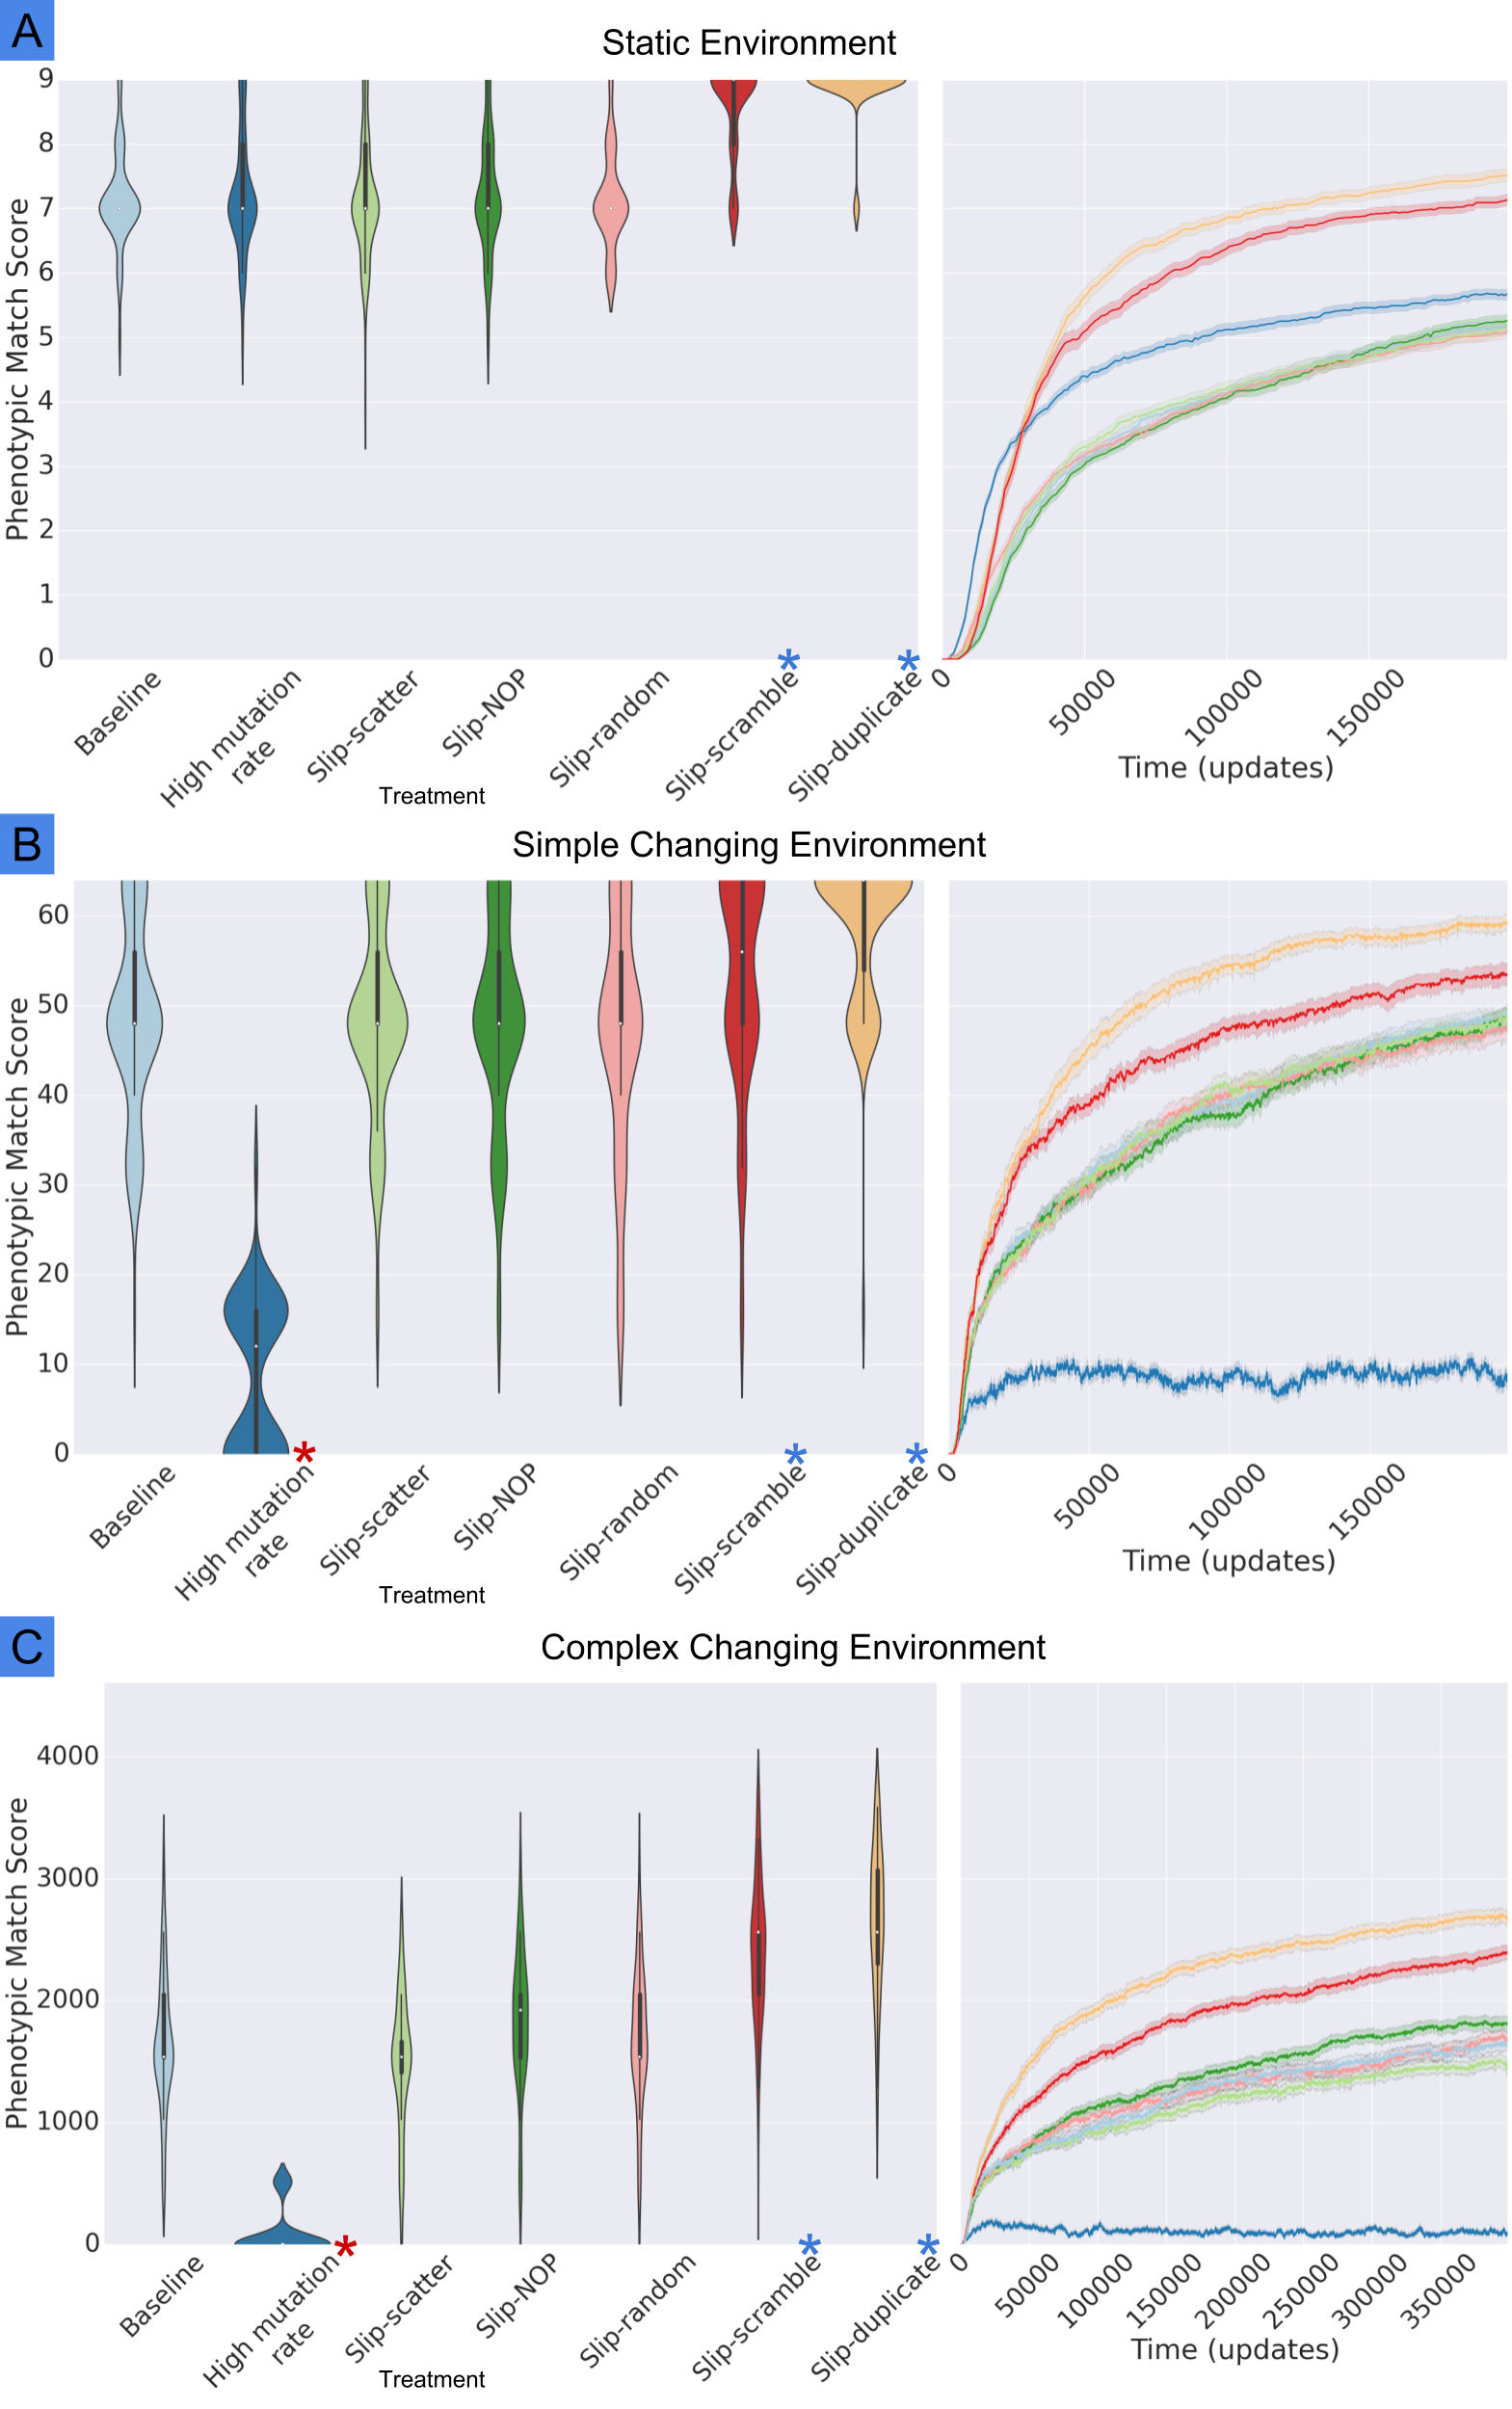
\includegraphics[width=\columnwidth]{imgs/results_panels.png}
  \caption{\small Experimental results from all three environments: A) static environment, B) simple changing environment, and C) complex changing environment. The violin plots for each environment indicate the phenotypic match scores for final dominants in the static environment and for the ancestors of final dominants that existed 1000 updates prior to the end of a trial in the simple and complex changing environments. Each time series shows the phenotypic match scores for the lineages of final dominant organisms over time. The colors in each time series correspond to the colors in the violin plots. Treatments that have significantly higher phenotypic match scores than the baseline treatment are marked with blue *, and treatments that have significantly lower phenotypic match scores than the baseline treatment are marked with red *.  }
  \label{fig:results_panels}
\end{figure}

\subsection{What configuration of gene duplication is most evolvable?}
Across all three environments
%(static, simple changing, and complex changing),
we found that the most important aspect of gene duplications is the capacity to duplicate meaningful information in the genome. As shown in Figure \ref{fig:results_panels}, %across all three environments,
only organisms that evolved in the slip-duplicate and slip-scramble treatments had significantly higher phenotypic match scores than organisms evolved in the baseline treatment.
Organisms evolved in all other experimental treatments were either not significantly different from the baseline treatment or significantly worse than the baseline treatment.

Of the five types of slip mutation operators used (see Figure \ref{fig:slip_mut_variants}), only the slip-duplicate and slip-scramble operators were capable of duplicating meaningful information in a genome.
Slip-scramble mutations maintain the content but not the ordering of duplicated instruction sequences; thus, they can duplicate information about what instructions make-up already successful genetic sequences but do not maintain the particular ordering of those instructions. Slip-duplicate mutations are the full form of gene duplication, %capable of duplicating even more information than slip-scramble mutations,
able to exactly duplicate the ordered instruction make-up of existing genetic sequences. In contrast to the slip-scramble and slip-duplicate operators, all other slip mutation operators do not duplicate information about instruction sequences already present in the genome.

Because the slip-scramble treatment was significantly better at promoting evolvability than the baseline treatment, we can conclude that the duplication of functional building blocks is valuable no matter how they are arranged when duplicated. However, is %duplicating more information better? Does it matter that gene duplications
it important to
preserve both the contents and ordering of duplicated sequences?

\subsubsection{Is more information better?}
From Figure \ref{fig:results_panels}, organisms evolved in the slip-duplicate treatment had higher phenotypic match scores than organisms evolved in the slip-scramble treatment, implying that the additional information in a gene duplication event %is able to replicate in a genome, the more it will
does
promote evolvability. To confirm this relationship and reduce multiple comparison issues with statistical tests, we re-ran 100 new trials of both the slip-duplicate and slip-scramble treatments %with new random number seeds
and compared the phenotypic match scores of the evolved organisms. In all three environments, organisms that evolved in the slip-duplicate treatment had significantly higher phenotypic match scores than organisms evolved in the slip-scramble treatment (two-tailed Mann-Whitney U tests, W = 4305, 4028.5, 3621.5 respectively, Bonferroni-adjusted $p$ values 0.0109, 0.0222, 0.0017, respectively). This result supports that %the capacity to duplicate more information is better, and the fact that gene duplications are capable of
duplicating both the content and structure of existing genetic code is an important factor in their ability to promote evolvability.

\subsection{Discerning the mechanism of slip duplication in facilitating adaptive evolution}

Having established slip-duplicate as the best-performing slip insertion operator, we next sought to understand the mechanism driving the evolvability impact of gene duplication in the Avida system.

One salient aspect of the task system in Avida is the hierarchical composition of task definitions.
``Simpler'' tasks like AND and NAND form the building blocks of the definition of ``more complex'' tasks like XOR and EQU.
In the past, this property has been applied to study the evolution of complex traits \citep{TODO}.
The complexity of the nine tasks used in this work can be approximted by the minimal number of NAND buliding blocks required to perform them\footnote{
In computer architecture theory, NAND is commonly established as the fundamental building block operation as all other logical operations are able to be derived from compositions of NAND gates \citep{TODO}.
},
\begin{enumerate}
\item NOT and NAND: one NAND component,
\item AND and ORNOT: two NAND components,
\item OR and ANDNOT: three NAND components,
\item NOR and XOR: four NAND components,
\item EQU: five NAND components.
\end{enumerate}
We exploited this natural hierarchy to test how gene duplication facilitated evolution across a spectrum of task complexity, by studying the rate at which different ``component count'' categories of tasks evolved.

One simple consequence of gene duplication is in increasing the number of sites in a genome.
We sought to identify the aspects of gene duplication evolvability that could be attributed simply to longer genome length.
For this purpose, we compared against an additional control, the long genome baseline control where genomes were 1,000 sites long.

Two alternate hypotheses can be understood about the role of gene duplication in adaptive evolution.
In one hypothesis, by facilitating greater robustness and redundancy.
This allows neofunctionalization and subfunctionalization.
In the fitness landscape analogy, this can be thought of as discovering the 

\subsubsection{Role of slip duplication in facilitating robustness and raw neutral genetic material.}

We found that instead of decreasing the amount of brittleness, genomes with slip duplications had comparable amounts of brittleness to the long-genome baseline treatment.
However, we found that the slip duplications provided a higher amount of previously coding material that was now neutral with respect to task performance.
So, in a sense a greater amount of coding material was available for neutral re-shaping even though overall robustness was not increased.

Under an alternate framing for role of gene duplication in facilitating evolution, gene duplication acts as a ``smart'' mutation operator that exploits information about the existing structure of the genome in order to increase the probability of directly discovering new adaptations.
This can be thought of as ``hopping'' to a new peak in fitness space.

We first investigated whether gene duplication increased genome robustness.
One definition of robustness is in terms of brittleness: the number of genome sites ``critical'' to fitness, where a single-site knockout caused the loss of one or more tasks.
We measured genome robstness through all-site knockouts using Avida's genome evaluator.

\begin{figure}
    \centering
    \begin{subfigure}{\linewidth}
    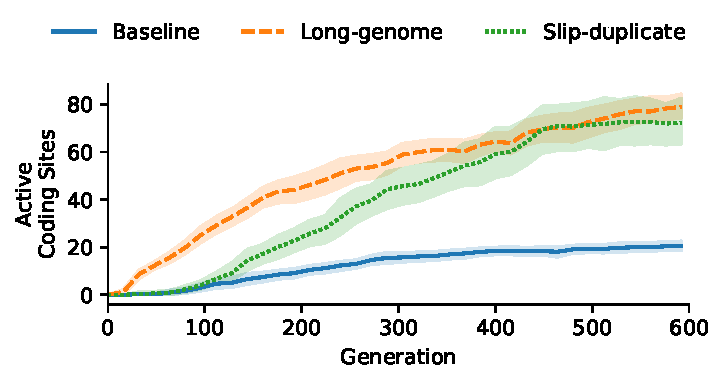
\includegraphics[width=\linewidth]{binder/binder/teeplots/hue=treatment+post=plt-xlim-0-600+viz=lineplot+x=generation-born+y=num-coding-sites+ext=.pdf}
    \caption{\footnotesize number coding sites (critical for tasks)}
    \label{fig:num-coding-sites:coding}
    \end{subfigure}

    \begin{subfigure}{\linewidth}
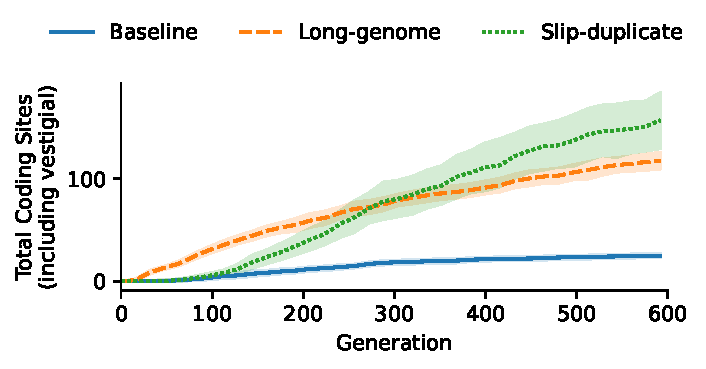
\includegraphics[width=\linewidth,]{binder/binder/teeplots/hue=treatment+post=plt-xlim-0-600+viz=lineplot+x=generation-born+y=num-coded-sites+ext=.pdf}
    \caption{\footnotesize number of sites that currently or have coded for a task}
    \label{fig:num-coding-sites:coded}
    \end{subfigure}
    \caption{
        \textbf{Growth trajectories of brittleness and coding site counts over evolutionary time.}
        \footnotesize
        Error bands give 95\% CI, bootstrapped over 30 replicates per treatment.
    }
    \label{fig:num-coding-sites}
\end{figure}



% https://github.com/chaynes2019/AvidaGeneDupe/blob/538ede79c7301f10718ca96c8dd38782b6882632/binder/num-coding-sites.ipynb
Figure \ref{fig:num-coding-sites} compares the trajectory of coding sites in genomes in slip-duplicate and control treatments over evolutionary generations.
We found that, at 600 generations, the long-baseline and slip-duplicate treatments did not differ significantly in their brittleness, measured as coding site count (Mann-Whitney U Test; Figure \ref{fig:num-coding-sites:coding}).
However, we found that they did differ in the raw amount of material that was or had previously been coding (Figure \ref{fig:num-coding-sites:coded}; $p < 0.0001$; Mann-Whitney U Test).
Thus, the slip-duplication increased the amount of potential material to work with but did not change the robustness \textit{per se}.

In additional experiments, we tested the effects of insertion mutations on brittleness (measured by coding site count) and found that neutral insertion mutations, indeed, do tend to reduce coding site count --- particularly for genomes with that encode high-complexity tasks (Supplementary Figure \ref{fig:nulldist}).
So, perhaps an evolutionary force is driving the two treatments to reach the same ballpark of critical sites, but the slip duplication can duplicate and copy around genome content in a manner that increases the copy count of previously-coding sites relative to the number of critical sites.

(It should be noted that this measure is limited, as it depends on functional sites being detectable at some point through single-site knockout which can fail to reveal aspects of sequence complexity \citep{alifeextendedabstract}.)

\subsubsection{Slip duplication specifically facilitates adaptive variation for the evolution of complex traits.}

\begin{figure*}
    \centering
    \begin{subfigure}{\textwidth}
    \includegraphics[width=\linewidth,trim={0 13cm 0 0},clip]{binder/binder/teeplots/adaptive-evolution-rate.ipynb/col=components+errorbar=ci+hue=treatment+kind=line+post=plt-xlim-0-600+row=mutation+viz=relplot+x=generation+y=has-task+ext=.pdf}
\includegraphics[width=\linewidth,trim={0 0 0 24cm},clip]{binder/binder/teeplots/adaptive-evolution-rate.ipynb/col=components+errorbar=ci+hue=treatment+kind=line+post=plt-xlim-0-600+row=mutation+viz=relplot+x=generation+y=has-task+ext=.pdf}
    \caption{\footnotesize including directly-facilitated adaptive variation from slip duplication (tasks gained directly through slip duplication); (blue: long-ancestor; purple: baseline treatment; orange: slip-duplicate treatment)}
    \label{fig:adaptive-evolution-rate:direct}
    \end{subfigure}

    \begin{subfigure}{\textwidth}
\includegraphics[width=\linewidth,trim={0 0 0 13cm},clip]{binder/binder/teeplots/adaptive-evolution-rate-nodirect.ipynb/col=components+errorbar=ci+hue=treatment+kind=line+post=plt-xlim-0-600+row=mutation+viz=relplot+x=generation+y=has-task+ext=.pdf}
    \caption{\footnotesize excluding directly-facilitated adpative variation from slip duplication (only instances where tasks did not arise as an immediate consequence of slip duplication); (brown: long-ancestor; purple: baseline treatment; red: slip-duplicate treatment)}
    \label{fig:adaptive-evolution-rate:nodirect}
    \end{subfigure}
    \caption{
        \textbf{Rate of adaptive evolution across a spectrum of task complexities.}
        \footnotesize
        Simple tasks (leftmost panels) require only one logic gate component.
        More complex tasks (rightmost panels) require up to five logic gate components.
        Slip-duplication treatment facilitates significantly faster adaptive evolution than long-genome treatment for more complex tasks, requiring 4 or 5 components (top panel).
        Without instances where tasks were acquired directly through slip duplicaiton, however, no significant difference is detected between the adaptive rates of long-genome and slip-duplication treatments for these more complex tasks (bottom panel).
        Error bands give 95\% CI, bootstrapped over 30 replicates per treatment.
    }
    \label{fig:adaptive-evolution-rate}
\end{figure*}


In a first set of experiments, we tested whether the adaptive boost of slip duplication was greater than the adaptive boost of simply having more genome sites.
Figure \ref{fig:adaptive-evolution-rate} shows the results of these experiments.

Genome length was sufficient to explain the boost to the rates at which simpler traits ($\leq 3$ components) were gained in the slip duplication treatment compared to the baseline treatment --- the long-genome baseline treatment indeed faster adaptive evolution of these traits compared to the slip-duplication treatment.
% https://github.com/chaynes2019/AvidaGeneDupe/blob/538ede79c7301f10718ca96c8dd38782b6882632/binder/adaptive-evolution-rate.ipynb
However, for 4 and 5 component traits, the slip-duplicate treatment had a significantly higher fraction of replicates that had evolved the these traits at 600 generations compared to the long genome control (exact Fisher tests; $p<0.05$ [4 components], $p < 0.03$ [5 components]; Figure \ref{fig:adaptive-evolution-rate:direct}).

% https://github.com/chaynes2019/AvidaGeneDupe/blob/538ede79c7301f10718ca96c8dd38782b6882632/binder/adaptive-evolution-rate-nodirect.ipynb
To assess whether such facilitation of robustness neutral variation described  was an important factor in explaining the adaptive boost of slip duplication, we tested whether a difference in adaptive rates was still detectable in the absence of directly-facilitated adaptive variation where slip duplications directly caused the gaining of new traits.
We found that this was not the case; without instances where new traits were directly discovered as the result of slip duplication, no significant difference remained in the adaptive evolution rate of the slip-duplicate and long-genome controls for the 4 and 5 component tasks (exact Fisher tests; Figure \ref{fig:adaptive-evolution-rate:nodirect}).

Thus, we can conclude that slip duplications are specific in facilitating the evolution of complex traits, but that facilitation of neutral variation --- as is commonly the narratie around gene duplication --- is not necessarily necessary to explain this phenomenon.

\subsection{Major Results}

In this work, we have found
\begin{itemize}
\item the most effective form of gene duplication in facilitating adaptive evolution within the Avida platform was the direct, local slip mutation;
\item increases in genome length appear sufficient to explain the role of slip duplication in facilitating adaptive evolution of simple traits, but slip duplication is uniquely facultative of evolution of complex traits;
\item we did not find evidence that slip duplication decreased genome brittleness; instead, slip duplication appears to increase the amount of ``play-dough'' neutral coding material in the genome;
\item slip duplication's effects in directly facilitating adaptive variation, as opposed to facilitating neutral variation, appears sufficient to explain its contribution to the evolution of complex traits in our experiments.
\end{itemize}

Much theoretical interest is paid to the role of gene duplication in facilitating neutral evolution, and opening the door for adaptive evolution of new complexity through subfunctionalization and neofunctionalization.
Indeed, ample evidence from experiments \textit{in silico} and \textit{in vivo} has been collected to support this view of the role of gene duplication in adpative evolution.

In contrast, our study highlights the important role of more direct and prosaic consequences of gene duplication: (1) in increasing the amount of raw sequence length available for mutation and selection to act on and (2) in directly facilitating variation by basing mutation off of existing genome content.

% \subsection{High mutation rate inhibits the evolution of regulation in changing environments}
% In addition to our results on why gene duplications promote evolvability, our experiments
% %demonstrate the potential for
% indicate that
% high mutation rates inhibit the evolution of regulation in changing environments. In both the simple and complex changing environments, organisms evolved in the high mutation rate treatment had significantly lower phenotypic match scores than organisms evolved in the baseline treatment, which can be seen in Figure \ref{fig:results_panels} (two-tailed Mann-Whitney U tests, W = 9958 and 9944, respectively, Bonferroni-adjusted $p$ values both $<< 0.0001$).
% A similar result was found in \citep{Lalejini:2016plasticity}. Although higher mutation rates increase genetic variation, most mutations have deleterious effects \citep{Schlichting:2002jl}. Thus, higher mutation rates may increase the difficulty of maintaining the genetic machinery necessary for complex regulation.

% If elevated mutation rates %can work to
% inhibit the evolution of regulation and all experimental treatments with slip mutation operators have an effectively higher mutation rate than the baseline treatment, why do we see this effect only in the high mutation rate treatment? The rates of insertions and deletions per instruction copied in the high mutation rate treatment were selected to, on average, result in approximately the same number of mutations per divide as in our treatments with slip mutations. Yet, only organisms evolved in the high mutation rate treatment had significantly lower phenotypic match scores than organisms evolved in the baseline treatment in the changing environments; all other experimental treatments were either significantly better or not significantly different than the baseline treatment.

% @amlalejini old text on mutation load explanation:
%Why is it that \textit{only} the high mutation rate treatment inhibited evolvability in the changing environments? One possibility is because slip mutations result in large mutational events that affect few offspring, whereas mutations in the high mutation rate treatment result in an increased number of smaller mutational events that are spread across many offspring. Thus, many offspring in the high mutation rate treatment are subject to the increased rate of deleterious mutations that results from an increase in the rates of copy insertions and copy deletions. This is in contrast to treatments with slip mutations where relatively fewer offspring are subjected to the increased rate of deleterious mutations because deleterious mutations are concentrated in a fewer offspring relative to the high mutation rate treatment.
%Further analysis is needed to confirm that this is, indeed, the case.
% @amlalejini new text on mutation load explanation:
%  - should I cite something for 'mutation load' (i.e. this concept exists, read about it here)?
% Why is it that \textit{only} the high mutation rate treatment inhibited evolvability in the changing environments?
% One possibility stems from the higher mutation load imposed on populations by the high mutation rate treatment.
% Slip mutations result in large mutational events that affect few offspring, whereas the elevated rate of copy mutations in the high mutation rate treatment results in an increased number of smaller mutational events spread across many offspring.
% Thus, many offspring in the high mutation rate treatment are subject to the increased rate of deleterious mutations that results from the higher rates of copy insertions and copy deletions. This is in contrast to treatments with slip mutations where relatively fewer offspring are subjected to large mutational events, which results in the concentration of deleterious mutations in fewer offspring relative to the high mutation rate treatment.
% Further analysis is needed to confirm that this is, indeed, the case.

% OLD figures
% \begin{figure}
    \centering
    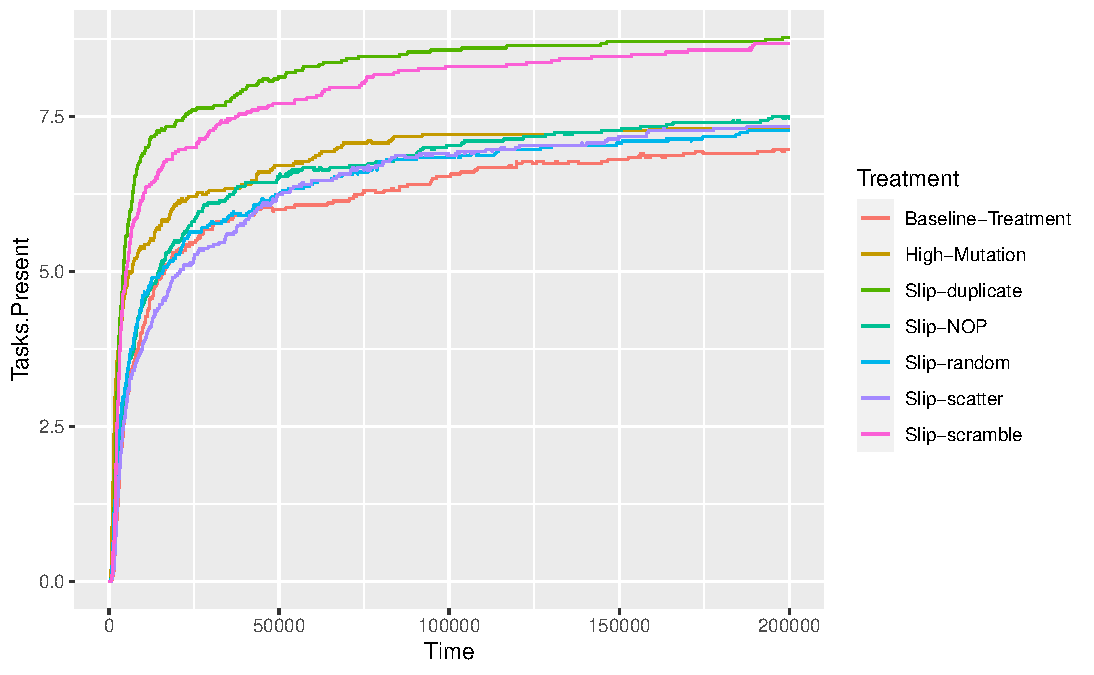
\includegraphics[width=\linewidth]{img/2022-3-29-PaperDuplication/TidiedData/FullReplicationTaskCountTimeCourse}
    \caption{TODO} \label{fig:FullReplicationTaskCountTimeCourse}
\end{figure}

% \begin{figure}
    \centering
    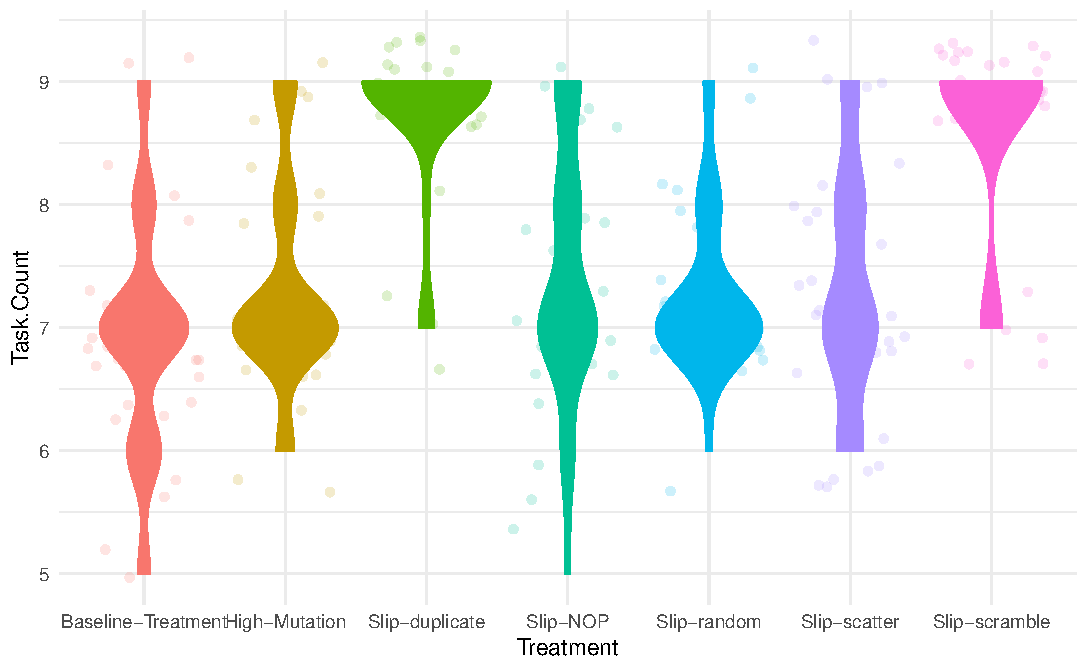
\includegraphics[width=\linewidth]{img/2022-3-29-PaperDuplication/TidiedData/FullReplicationFinalDominantTaskCountViolin}
    \caption{TODO} \label{fig:FullReplicationFinalDominantTaskCountViolin}
\end{figure}

% \begin{figure}
    \centering
    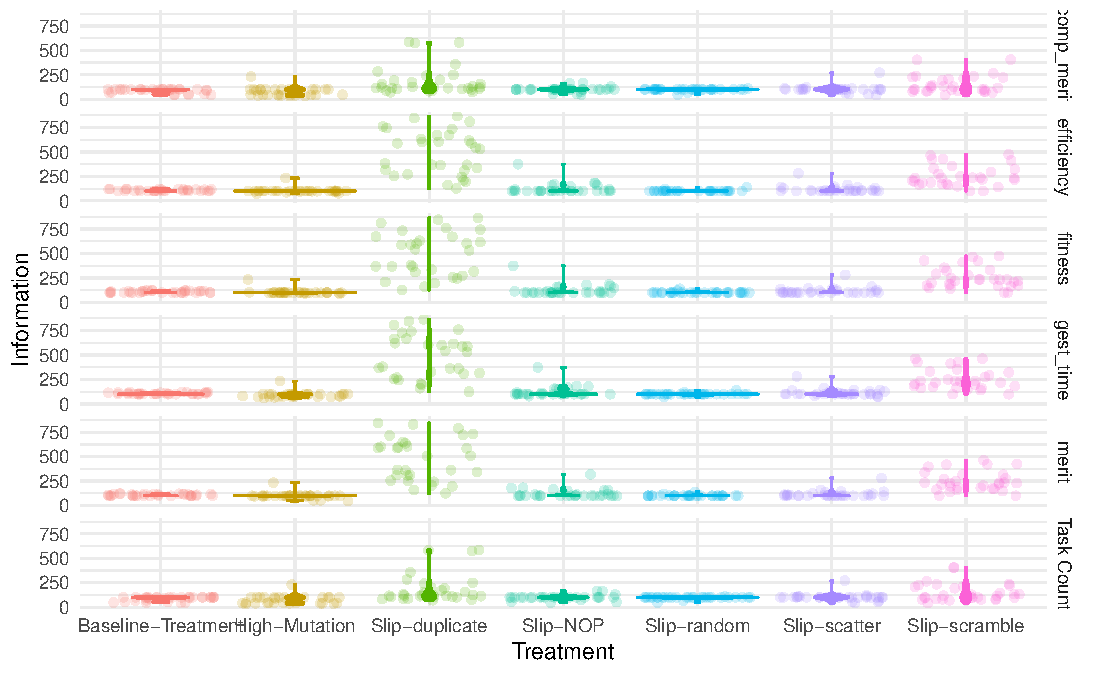
\includegraphics[width=\linewidth]{img/2022-3-29-PaperDuplication/TidiedData/LalejiniEtAlReplicationFinalDominantInfo}
    \caption{TODO} \label{fig:LalejiniEtAlReplicationFinalDominantInfo}
\end{figure}

% \begin{figure}
    \centering
    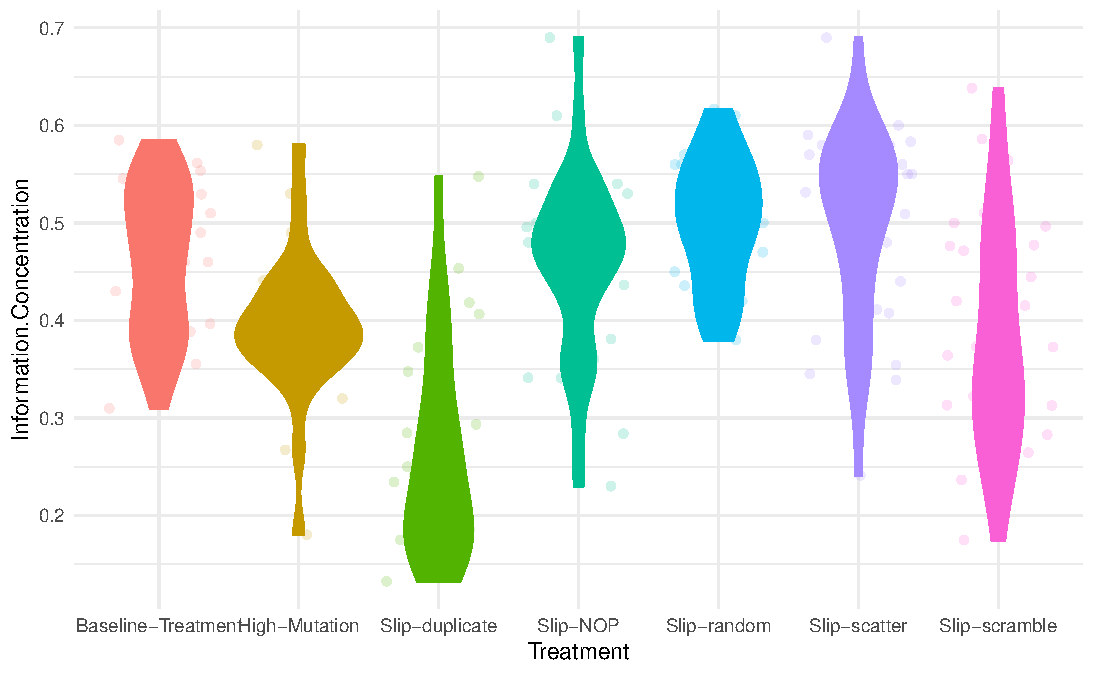
\includegraphics[width=\linewidth]{img/2022-3-29-PaperDuplication/TidiedData/LalejiniEtAlReplicationFinalDominantInfoConcentration}
    \caption{TODO} \label{fig:LalejiniEtAlReplicationFinalDominantInfoConcentration}
\end{figure}

% \begin{figure}
    \centering
    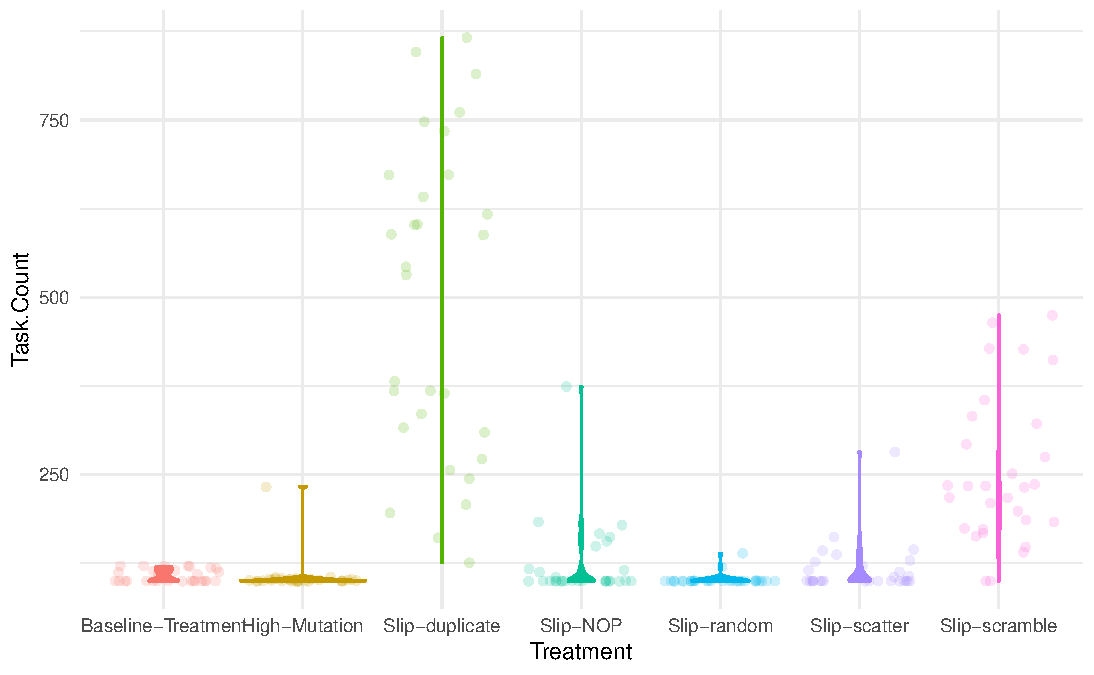
\includegraphics[width=\linewidth]{img/2022-3-29-PaperDuplication/TidiedData/LalejiniEtAlReplicationFinalDominantGenomeLengthsViolin}
    \caption{TODO} \label{fig:LalejiniEtAlReplicationFinalDominantGenomeLengthsViolin}
\end{figure}

% \begin{figure}
    \centering
    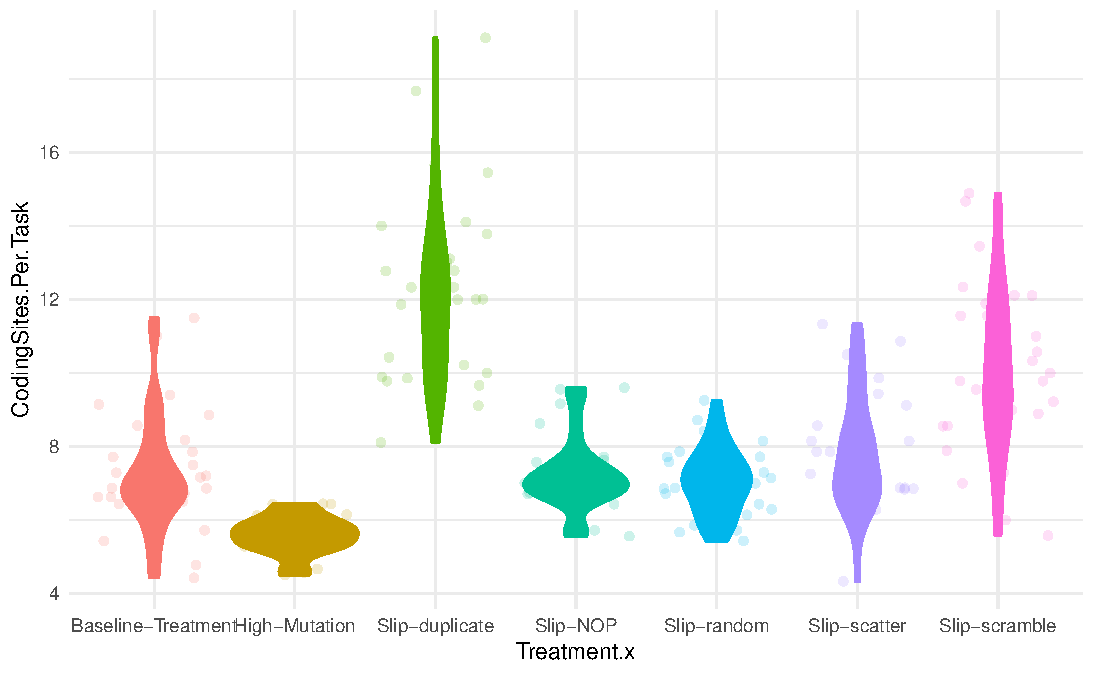
\includegraphics[width=\linewidth]{img/2022-3-29-PaperDuplication/TidiedData/LalejiniEtAlReplicationFinalDominantCodingSitesPerTask}
    \caption{TODO} \label{fig:LalejiniEtAlReplicationFinalDominantCodingSitesPerTask}
\end{figure}

% \begin{figure}
    \centering
    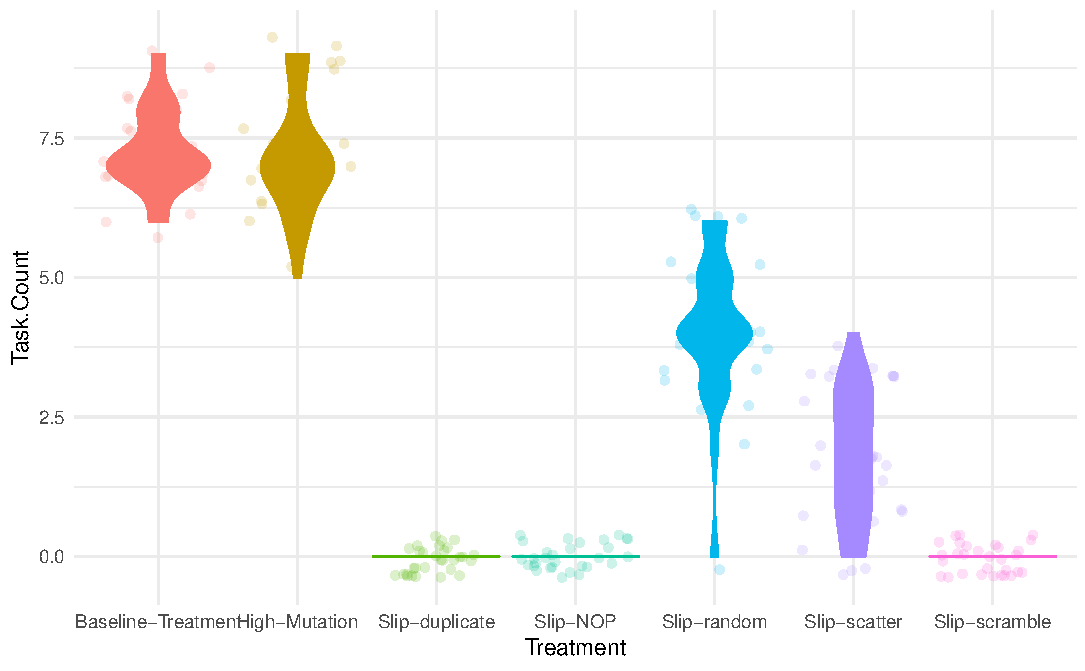
\includegraphics[width=\linewidth]{img/2022-3-29-PaperDuplication/TidiedData/ModifiedReplicationFinalDominantTaskCountViolin}
    \caption{TODO} \label{fig:ModifiedReplicationFinalDominantTaskCountViolin}
\end{figure}

% \begin{figure}
    \centering
    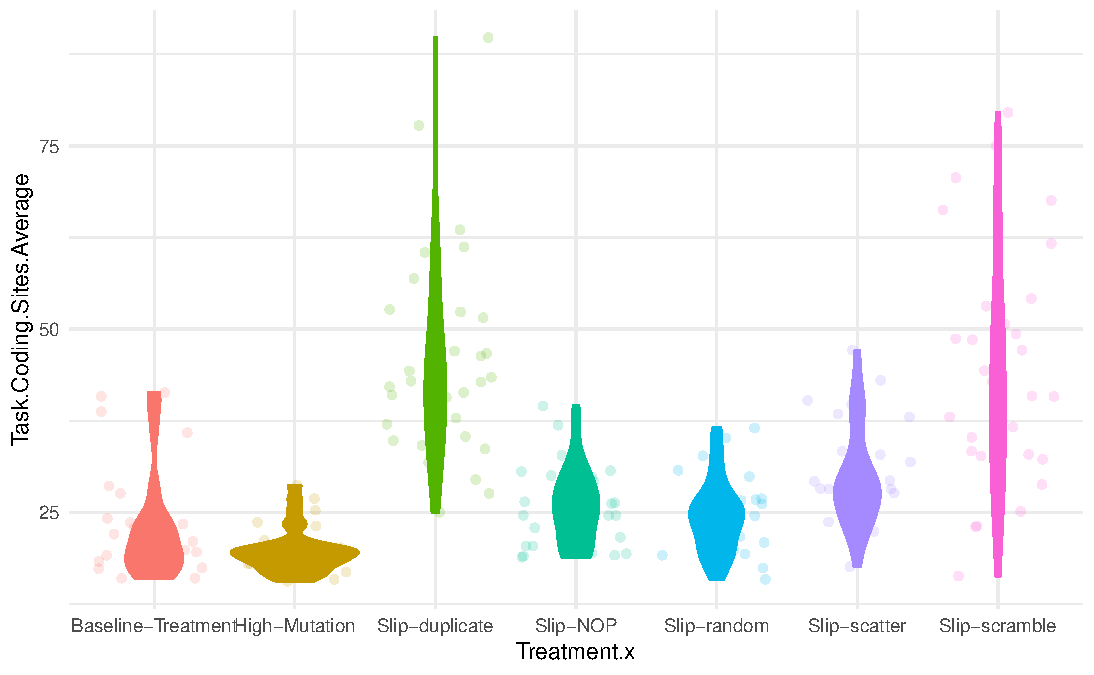
\includegraphics[width=\linewidth]{img/2022-3-29-PaperDuplication/TidiedData/LalejiniEtAlReplicationRealFinalDominantCodingSitesPerTask}
    \caption{TODO} \label{fig:LalejiniEtAlReplicationRealFinalDominantCodingSitesPerTask}
\end{figure}

% \begin{figure}
    \centering
    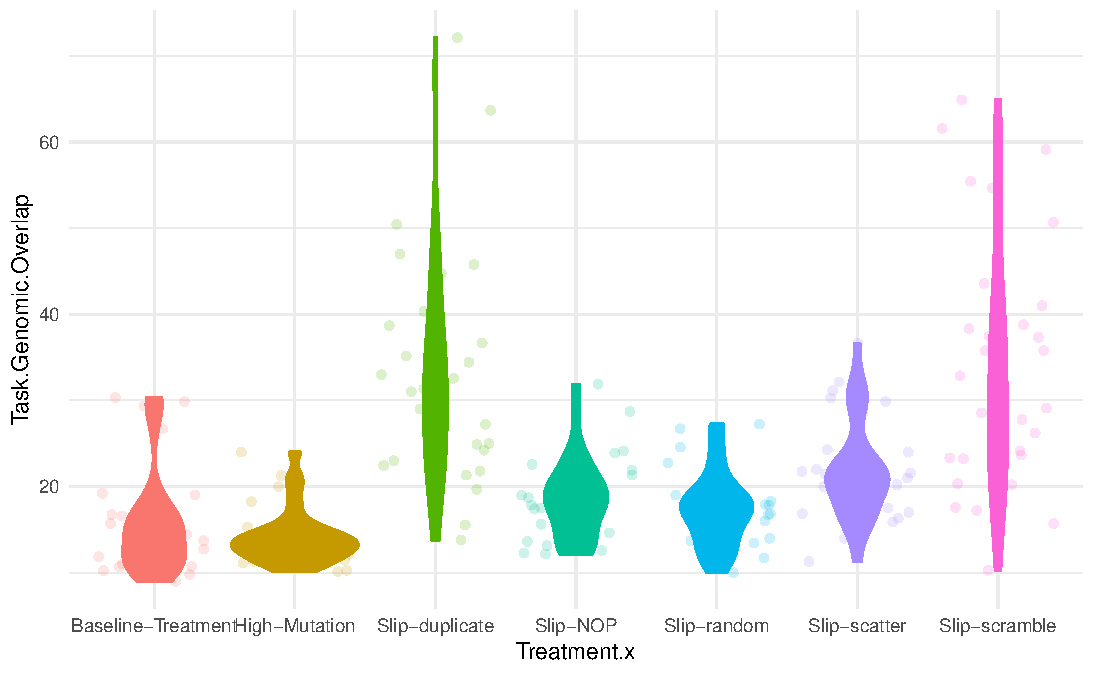
\includegraphics[width=\linewidth]{img/2022-3-29-PaperDuplication/TidiedData/LalejiniEtAlReplicationFinalDominantOverlap}
    \caption{TODO} \label{fig:LalejiniEtAlReplicationFinalDominantOverlap}
\end{figure}

